\clearpage
\section{Event Selection\label{sec:eventSelection}}

As discussed in section~\ref{sec:SUSY}, all-hadronic SUSY signatures consist of events with
no isolated and detectable objects apart from energetic jets. One can quantify the
total visible energy in these type of events with the quantity, \scalht, the sum of 
the transverse energy of the jets in the event. The challenges due to large
backgrounds in a search for an excess in all-hadronic events becomes evident 
when comparing observed data events overlaid with simulated events from 
SM processes as a function of \scalht, figure~\ref{fig:HT-distribution}.

\begin{figure}[h!t]
  \begin{center}
      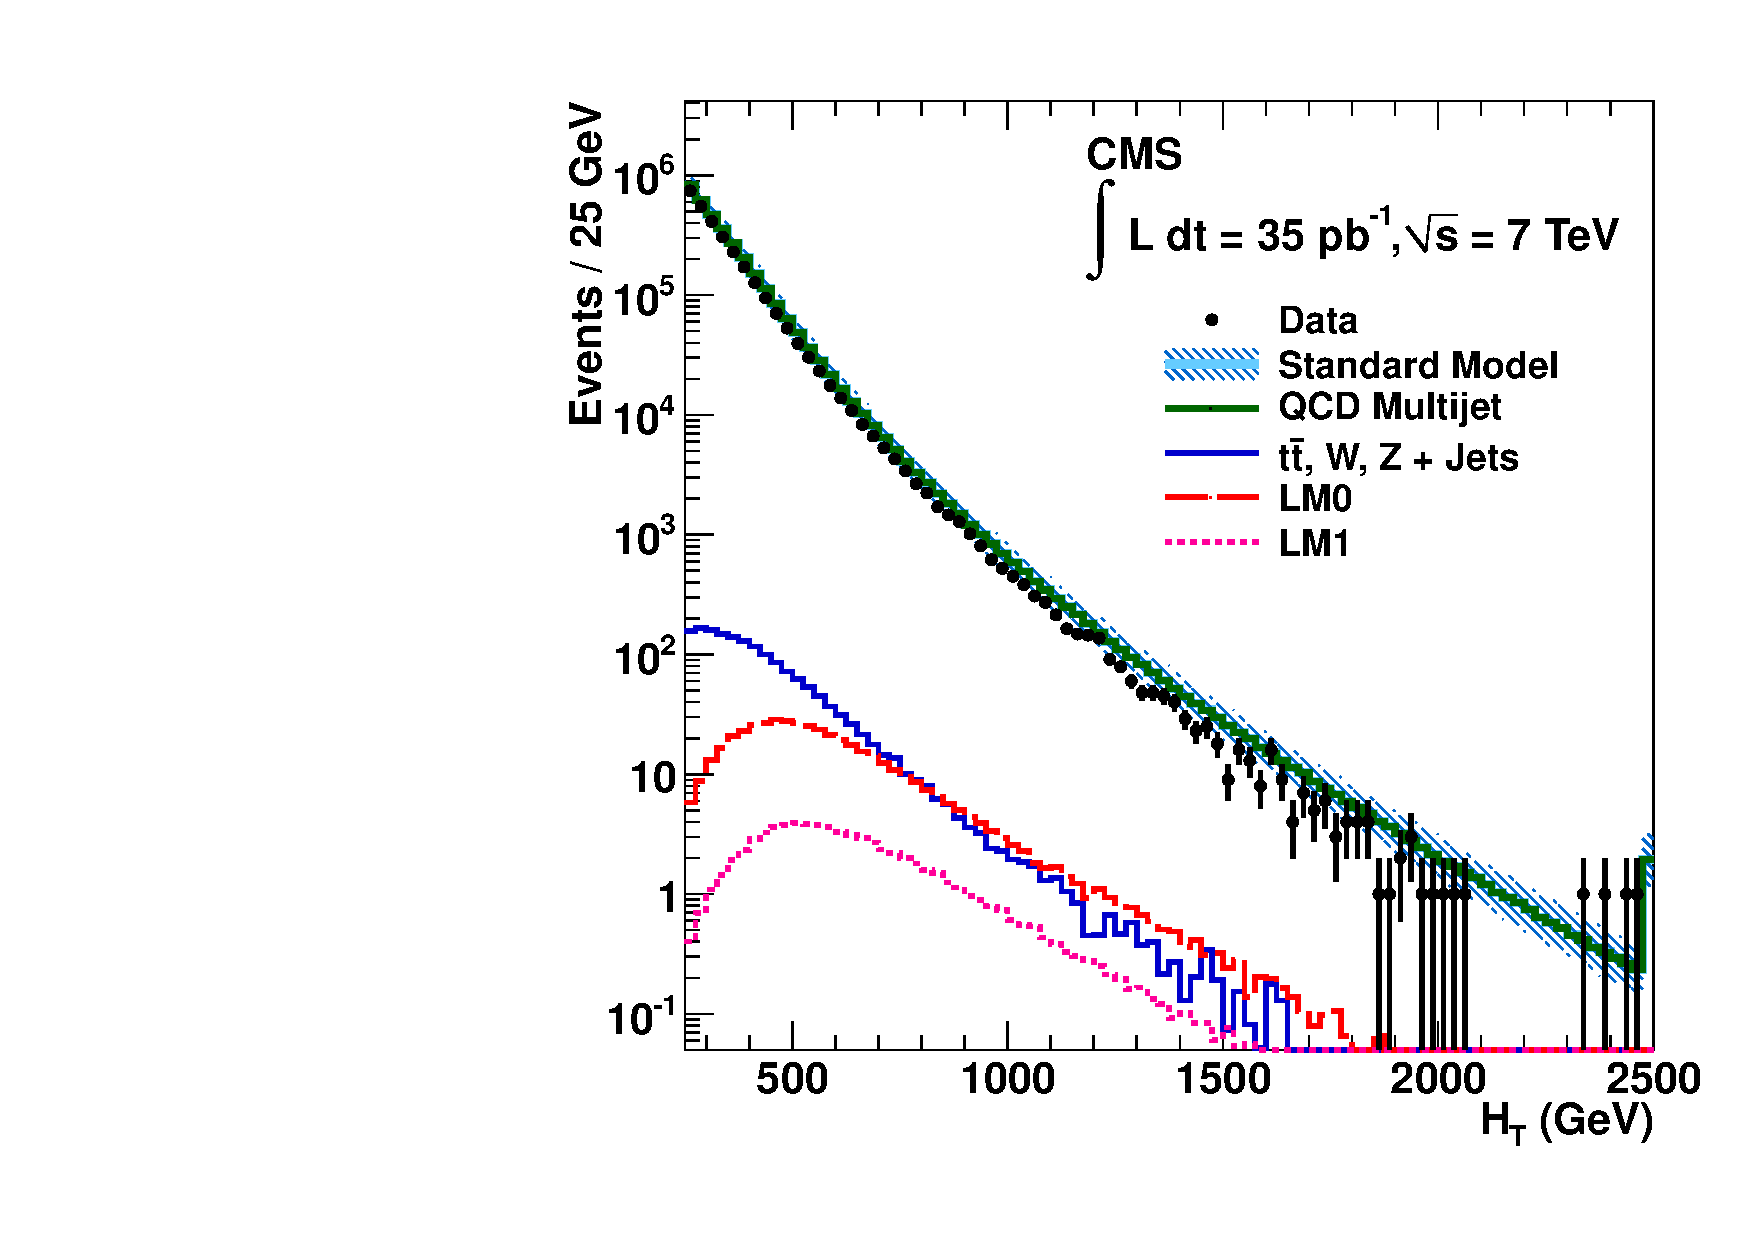
\includegraphics[width=0.45\textwidth,]{figures/data-mc/AllcombinedHT_all.pdf}
      \caption{\label{fig:ht} $\scalht$ distribution after basic preselection,
           for 35~pb$^{-1}$ of data collected at {7}~\tev as well as for all 
           standard model backgrounds and two SUSY signal samples, from~\cite{RA1Paper}. 
           This figure is for illustrative purposes only, as these specific SUSY 
           models are not under study in this analysis}
    \label{fig:HT-distribution}
  \end{center}
\end{figure}

The dominant background are azimuthally-balanced (i.e. back-to-back in the azimuthal angle 
$\phi$) multi-jet events, stemming from QCD processes. This search reduces this background 
to negligible levels in the hadronic search region by employing the \alphat variable further 
discussed in section~\ref{sec:alphat}. Furthermore, by construction, \alphat also reduces 
backgrounds from mis-measured back-to-back jets. In absence of the multi-jet QCD events,
the remaining significant backgrounds are SM process with genuine \met. The expected 
yield of these backgrounds are measured using two control samples. The following sections
describe the identification of objects used in the hadronic and control samples, while the 
detailed description of the background and control samples are left for 
chapter~\ref{sec:background}.

\subsection{Data}
The data analyzed was recorded by CMS in 2012 between April 5th and Dec. 5th and
totals 19.47$\pm$ 2.6\%. The collected data is certified on a run-by-run 
basis, where initial automatic certification requires the LHC beams to be declared
stable and all CMS subdetectors ON. Further monitoring of the data was done real time
by experts of each subdetector trough analysis of histograms updated and filled
each lumi section. Final certification was done offline, and lumi sections passing
all criteria were listed in a Golden JSON file to be used by all analyses. 

\subsection{Event quality}

Each event is subjected to a series of commonly used filters in CMS to ensure good
quality data. Minimal requirements are that at least one primary vertex is identified 
and 25\% of the reconstructed tracks to be of good quality. Additionally, various filters 
prescribed by the MET group[REF] are applied. Events containing muons with inconsistent
energy are flagged by the muon pog [REF] and filtered out of the analysis. 

\clearpage
\section{Physics objects\label{sec:reconstruction}}

The definitions of the physics objects used in this analysis follow
the recommendations of the various Physics Object Groups (POGs).

\subsection{Jets}

Jets are reconstructed by combining information from multiple
sub-detectors using the Particle-Flow (PF) algorithm~\cite{PAS-PFT-09-001} 
and clustered by the anti-$k_{\rm T}$ algorithm~\cite{antikt} with
a size parameter of $0.5$. Three levels of jet energy corrections are 
applied; level 1 corrects for overlapping pp collisions 
(pile-up ~\cite{Cacciari2008119,1126-6708-2008-04-005}) in the jet, 
level 2 and 3 correct the jet energy response to be $\eta$ and $\pt$ independent.  
Further residual corrections are applied on data which correct for 
small remaining discripencies in the modelling of the response. The acceptance of
``fake'' jets is supressed by requring that jets pass jet identitifcation at the 
Loose working point~\cite{ref:jet-id}. This requires that the jet is comprised
of more than one particle and that those particles cannot all be neutral hadrons 
(i.e. neutrons) or all neutral particle deposits in the ECAL (i.e. photons).
Additionaly if the jet is reconstructed outside outside the tracker's 
instrumatation, the jet is required to have more than one charged 
constituent, of which not all of them deposit their energy in the ECAL. 
Only jets reconstructed within the calorimeters' barrel and endcap, 
i.e. $|\eta| <$ 3.0, and with transverse momentum $\pt >$ 50\gev  
are considered in the analysis. Jets originating from bottom quarks 
(b-jets) are identified through vertices that are displaced with respect to the primary 
interaction~\cite{CMS-PAS-BTV-12-001}. The algorithm used to tag b-jets 
is the Combined Secondary Vertex tagger, using the "Medium" working point, 
which is achieved by requiring a cut of $>$0.679 on the algorithm discriminator 
variable and results in a gluon/light-quark quark mis-tag rate of 1\% 
(where ``light'' means $u$, $d$ and $s$ quarks) and an efficiency in the 
range $60-70\%$ depending on the jet \pt. 

\subsection{Muons}

Muons are identified according to the Tight working point definition
($\sim$95\% efficiency) of the muon identification
algorithm~\cite{ref:muon-id}. The algorithm works to reject cosmic muons or 
muons from decays in flight for consideration in the analysis. 
A PF-based ``combined relative'' isolation~\cite{ref:muon-id} is determined 
within a cone size $\Delta R < 0.4$, and "$\Delta\beta$" corrections 
are applied to remove the effects of pileup. Table~\ref{tab:muon-id} summarizes the
identification and isolation requirements. 
%This object is used as a
%veto as part of the hadronic signal region definition, as described in
%Section~\ref{sec:vetoes}, and as part of the \mj control
%sample selection described in Section~\ref{sec:def-control-samples}.

\begin{table}[h!]
  \caption{Muon identification (Tight working point).\label{tab:muon-id}}
  \centering
  \footnotesize
  \begin{tabular}{ lc }
    \hline
    \hline
    Global Muon                            & True      \\
    PFMuon                                 & True      \\
    $\chi^{2}$ fit                         & $<10$     \\
    Muon chamber hits                      & $>0$      \\
    Muon station hits                      & $>1$      \\
    Transverse impact $d_{xy}$             & $<0.2\mm$ \\
    Longitudinal dist $d_{z}$              & $<0.5\mm$ \\
    Pixel hits                             & $>0$      \\
    Track layer hits                       & $>5$      \\
    PF Isolation ($\Delta\beta$ corrected) & $<0.12$   \\
    \hline
    \hline
  \end{tabular}
\end{table}

\subsection{Photons}
%
Selected photons must satisfy the Tight working point definition 
($\sim$70\% efficiency) of the simple cut-based photon identification
algorithm~\cite{ref:photon-id-egamma}. Pile-up corrected isolation is 
determined within a cone size $\Delta R < 0.3$ using the PF-based 
isolation algorithm~\cite{ref:photon-id-egamma}. 
Table~\ref{tab:photon-id-egamma} summarises the identification
and isolation requirements. 

\begin{table}[ht!]
  \caption{Photon identification (Tight working point).\label{tab:photon-id-egamma}}
  \centering
  \footnotesize
  \begin{tabular}{ ccc }
    \hline
    \hline
    Categories                    & Barrel                             & EndCap                             \\
    \hline
    Conversion safe electron veto & Yes                                & Yes                                \\
    Single Tower H/E              & 0.05                               & 0.05                               \\
    $\sigma_{i\eta i\eta}$        & 0.11                               & 0.31                               \\
    PF charged hadron isolation   & 0.70                               & 0.50                               \\
    PF neutral hadron isolation   & 0.4 + 0.04 $\times$ $\pt^{\gamma}$  & 1.5 + 0.04 $\times$ $\pt^{\gamma}$  \\
    PF photon isolation           & 0.5 + 0.005 $\times$ $\pt^{\gamma}$ & 1.0 + 0.005 $\times$ $\pt^{\gamma}$ \\
    \hline
    \hline
  \end{tabular}
\end{table}

\subsection{Electrons}

Electrons are identified according to the Veto working point
definition ($\sim$95\% efficiency) of the cut-based \verb!Egamma!
identification algorithm~\cite{ref:electron-id}. PF-based
isolation~\cite{ref:electron-isolation} is determined within a cone
size $\Delta R < 0.3$ and $\rho \times A_{\textrm{eff}}$ corrections
are applied to remove the effects of pileup. Table~\ref{tab:ele-id}
summarises the identification and isolation requirements. 
%This object
%is used as a veto as part of the hadronic signal region definition, as
%described in Section~\ref{sec:vetoes}.

\begin{table}[h!]
  \caption{Electron identification (Loose working point).\label{tab:ele-id}}
  \centering
  \footnotesize
  \begin{tabular}{ lcc }
    \hline
    \hline
    Categories                                               & Barrel    & EndCap    \\
    \hline
    $\Delta \eta_{In}$                                       & 0.007     & 0.009     \\
    $\Delta \phi_{In}$                                       & 0.15      & 0.10      \\
    $\sigma_{i\eta i\eta}$                                   & 0.01      & 0.03      \\
    H/E                                                      & 0.12      & 0.10      \\
    d0 (vtx)                                                 & 0.02      & 0.02      \\
    dZ (vtx)                                                 & 0.2       & 0.20      \\
    $\lvert(1/E_{\textrm{ECAL}} - 1/p_{\textrm{trk}})\rvert$ & 0.05      & 0.05      \\
    PF relative isolation                                    & 0.15      & 0.15      \\
    Vertex fit probability                                   & 10$^{-6}$ & 10$^{-6}$ \\
    Missing hits                                             & 1         & 1         \\
    \hline
    \hline
  \end{tabular}
\end{table}

%\subsection{Single isolated tracks}
%W boson can be identified if they
%Leptonic decay products of W bosons will leave one single isolated track (SIT) 
%in the tracker. A single isolated track (SIT) can be used to identify W bosons through
%their leptonic decays: $\textrm{W} \ra \mu \nu$, $\textrm{W} \ra e
%\nu$, and $\textrm{W} \ra \tau (\ra \ell) \nu$. Also, single prong
%decays of the tau lepton can be identified: $\textrm{W} \ra \tau (\ra
%h^{\pm} + n\pi^{0})\nu$. A single isolated track comprises a charged
%PF candidate that satisfies the requirements listed in
%Table~\ref{tab:sit-id}. The relative track isolation is determined
%from the vectorial sum of neighbouring charged PF candidates within a
%cone $\Delta R < 0.3$ and satisfying $\Delta z (\textrm{candidate,PV})
%< 0.05\cm$ around the candidate isolated track. This object can be
%used to efficiently suppress the ``lost lepton'' background from W and
%\ttbar, as described in Section~\ref{sec:vetoes}. This definition is
%based on the one used in SUS-13-011 (``single lepton stop search with
%transverse mass'')~\cite{singleleptonstop}.
%
%\begin{table}[h!]
%  \caption{Single isolated track identification.\label{tab:sit-id}}
%  \centering
%  \footnotesize
%  \begin{tabular}{ lc }
%    \hline
%    \hline
%    Track \Pt                      & $>10\gev$  \\
%    $\Delta z (\textrm{track,PV})$ & $<0.05\cm$ \\
%    Charge                         & $\neq 0$   \\
%    Relative track isolation       & $<0.1$     \\
%    \hline
%    \hline
%  \end{tabular}
%\end{table}
%
%\subsection{Missing transverse energy}
%
%Missing transverse energy, \met, is defined by the type-I corrected
%particle-flow (PF)-based MET algorithm~\cite{ref:MET-corrections}. The
%\met variable is only used in the following two cases: to define of
%the tranverse mass variable, \mt, which is in turn used as part of the
%selection criteria that define the \mj control sample, described in
%Section~\ref{sec:def-control-samples}; to define a cleaning filter
%applied after the \alphat requirement, as described in
%Section~\ref{sec:had-signal}.


\subsection{Triggers}

\subsubsection{Hadronic signal region and control samples\label{sec:signal_triggers}} 

Only events passing one or more HLT triggers based on online quantities 
are recorded to be analyzed. For any analysis, in general, it is 
not expected that all recorded events reconstructed offline, pass the online
trigger as detector conditions, energy corrections, and object-based quantities
differ offline. In this analysis, cross-triggers at the HLT
based on quantities \scalht and \alphat (labeled as \verb!HTxxx_AlphaT0pyy!) 
are used with various thresholds to record candidate events for the hadronic (signal)
region. In order to keep the cross-trigger's computational time low, the online quantities
are constructed using calorimeter based jets (calo jets), and the use of
particle-flow jets in this analysis is expected to introduce inefficiencies.

Each \scalht bin is seeded by a single trigger chosen based on the
efficiency of the trigger in that \scalht bin. The \alphat thresholds of the
\verb!HTxxx_AlphaT0pyy! triggers were tuned according to the threshold
on the \scalht leg in order to fully suppress QCD multijet events~\cite{RA1Paper2012}
and simultaneously satisfying other criteria, such as maintaining
acceptable trigger rates.



%Table~\ref{tab:htalphat-triggers} summarises the thresholds used for
%the \verb!HTxxx_AlphaT0pyy! triggers. 
%
The \verb!HTxxx_AlphaT0pyy! trigger efficiencies are measured with a
reference (\ie, unbiased) event sample recorded by an unprescaled,
loosely-isolated, eta-restricted single muon 
trigger, \verb!HLT_IsoMu24_eta2p1!, within the \verb!SingleMu! dataset. A
sample of events containing at least one isolated muon with $\pt >
25\gev$ and $|\eta| < 2.1$ is used (similar to the \mj control sample
defined in Section~\ref{sec:def-control-samples}). A cut of $\Delta
{\rm R} > 0.5$ is placed between all muons and jets in each event, and
only jets are considered in the calculation of \scalht, \mht, and
\alphat, \ie the muon is ignored.

\begin{table}[!h]
  \caption{List of signal triggers and their efficiencies (\%), as
    measured in data. The trigger efficiency is $\sim$100\% for all
    bins above $\scalht > 675\gev$.}  
  \label{tab:htalphat-triggers}
  \centering
  \footnotesize
  \begin{tabular}{ cccccc }
    \hline
    \hline
    Offline \scalht       & Offline \alphat & L1 seed (\verb!L1_?!)         & Trigger (\verb!HLT_?!)  & \multicolumn{2}{c}{Efficiency (\%)}          \\ [0.5ex]
    region (\gev)         & threshold       & (highest thresholds)          &                         & $2 \leq \njet \leq 3$ & $\njet \geq 4$       \\ [0.5ex]
    \hline
    %$200 < \scalht < 275$ & 0.65            & \verb!DoubleJetC64!           & \verb!HT200_AlphaT0p57! & $81.8^{+0.4}_{-0.4}$  & $78.9^{+0.3}_{-0.4}$ \\
    %$275 < \scalht < 325$ & 0.60            & \verb!DoubleJetC64!           & \verb!HT200_AlphaT0p57! & $95.2^{+0.3}_{-0.4}$  & $90.0^{+1.2}_{-1.3}$ \\
    %$325 < \scalht < 375$ & 0.55            & \verb!DoubleJetC64 OR HTT175! & \verb!HT300_AlphaT0p53! & $97.9^{+0.3}_{-0.3}$  & $95.6^{+0.9}_{-1.0}$ \\
    $375 < \scalht < 475$ & 0.55            & \verb!DoubleJetC64 OR HTT175! & \verb!HT300_AlphaT0p53! & $94.2^{+0.5}_{-0.6}$  & $90.5^{+1.2}_{-1.3}$ \\
    $475 < \scalht < 575$ & 0.55            & \verb!DoubleJetC64 OR HTT175! & \verb!HT350_AlphaT0p52! & $96.2^{+0.8}_{-0.9}$  & $94.6^{+1.2}_{-1.4}$ \\
    $575 < \scalht < 675$ & 0.55            & \verb!DoubleJetC64 OR HTT175! & \verb!HT400_AlphaT0p51! & $95.4^{+1.4}_{-1.8}$  & $98.7^{+0.7}_{-1.12}$ \\
    $\scalht > 675$       & 0.55            & \verb!DoubleJetC64 OR HTT175! & \verb!HT400_AlphaT0p51! & $100^{+0.0}_{-2.0}$  & $100^{+0.0}_{-2.0}$ \\
    \hline
    \hline
  \end{tabular}
\end{table}


Table~\ref{tab:htalphat-triggers} summarizes the measured efficiencies
for the \verb!HTxxx_AlphaT0pyy! triggers in the relevant \scalht
bins. The trigger efficiencies are measured for both \njet
multiplicity bins. %The efficiencies are generally observed to be high,
%$\sim$100\%, except for the low \scalht region $200 < \scalht <
%325\gev$. The inefficiencies at low \scalht are mainly due to the L1
seeds for which thresholds were raised to a relatively high level in
order to maintain trigger rates in the high-pileup conditions towards
the end of Run 1. The inefficiencies are slightly larger in the higher
jet multiplicity category due to a larger number of jets summing to
the same \scalht, resulting in softer
jets. Figures~\ref{fig:eff-alphat-le3j} and~\ref{fig:eff-alphat-ge4j}
show the efficiency curves for the \verb!HTxxx_AlphaT0pyy! triggers in
the three lowest \scalht bins, for the \njetlow and \njethigh
categories, respectively. The efficiencies are also determined at the
level of event categories and no dependence on \nb is observed, with
efficiencies agreeing within statistical uncertainties.


\begin{figure}[!h]
  \begin{center}
    \subfigure[\njetlow, $375 < \scalht < 475 \gev$]{
      
\includegraphics[width=0.4\textwidth,page=30]{figures/trigger/plotDump/v29/HT375_475_100_100_50_AlphaT_HT300xaT0p53_PF_le3j_RunAtFNAL.pdf}
    }
    \subfigure[\njethigh, $375 < \scalht < 475 \gev$]{
      
\includegraphics[width=0.4\textwidth,page=30]{figures/trigger/plotDump/v29/HT375_475_100_100_50_AlphaT_HT300xaT0p53_PF_ge4j_RunAtFNAL.pdf}
    } \\
    \subfigure[\njetlow, $475 < \scalht < 525 \gev$]{
      
\includegraphics[width=0.4\textwidth,page=30]{figures/trigger/plotDump/v29/HT475_575_100_100_50_AlphaT_HT350xaT0p52_PF_le3j_RunAtFNAL.pdf}
    } 
    \subfigure[\njethigh, $475 < \scalht < 525 \gev$]{
      
\includegraphics[width=0.4\textwidth,page=30]{figures/trigger/plotDump/v29/HT475_575_100_100_50_AlphaT_HT350xaT0p52_PF_ge4j_RunAtFNAL.pdf}
    } \\
    \subfigure[\njetlow, $525 < \scalht < 675 \gev$]{
      
\includegraphics[width=0.4\textwidth,page=27]{figures/trigger/plotDump/v29/HT575_675_100_100_50_AlphaT_HT400xaT0p51_PF_ge4j_RunAtFNAL.pdf}
    }
    \subfigure[\njethigh, $525 < \scalht < 675 \gev$]{
      
\includegraphics[width=0.4\textwidth,page=27]{figures/trigger/plotDump/v29/HT575_675_100_100_50_AlphaT_HT400xaT0p51_PF_ge4j_RunAtFNAL.pdf}
    } \\
    \caption{\label{fig:eff-alphat-le3j}
      Cumulative efficiency turn-on curves for the \scalht-\alphat 
      cross triggers (as summarized in Table~\ref{tab:htalphat-triggers}) 
      that record events for the three lowest \scalht bins for events 
      satisfying \njetlow (left) and \njethigh (right). 
    }
  \end{center}
\end{figure}
%
%\begin{figure}[!h]
%  \begin{center}
%    \subfigure[Differential, $375 < \scalht < 475 \gev$]{
%      
\includegraphics[width=0.4\textwidth,page=20]{figures/trigger/plotDump/v29/HT375_475_100_100_50_AlphaT_HT300xaT0p53_PF_le3j_RunAtFNAL.pdf}
%    }
%    \subfigure[Cumulative, $375 < \scalht < 475 \gev$]{
%      
\includegraphics[width=0.4\textwidth,page=30]{figures/trigger/plotDump/v29/HT375_475_100_100_50_AlphaT_HT300xaT0p53_PF_le3j_RunAtFNAL.pdf}
%    } \\
%    \subfigure[Differential, $475 < \scalht < 525 \gev$]{
%      
\includegraphics[width=0.4\textwidth,page=20]{figures/trigger/plotDump/v29/HT475_575_100_100_50_AlphaT_HT350xaT0p52_PF_le3j_RunAtFNAL.pdf}
%    } 
%    \subfigure[Cumulative, $475 < \scalht < 525 \gev$]{
%      
\includegraphics[width=0.4\textwidth,page=30]{figures/trigger/plotDump/v29/HT475_575_100_100_50_AlphaT_HT350xaT0p52_PF_le3j_RunAtFNAL.pdf}
%    } \\
%    \subfigure[Differential, $525 < \scalht < 675 \gev$]{
%      
\includegraphics[width=0.4\textwidth,page=18]{figures/trigger/plotDump/v29/HT575_675_100_100_50_AlphaT_HT400xaT0p51_PF_le3j_RunAtFNAL.pdf}
%    }
%    \subfigure[Cumulative, $525 < \scalht < 675 \gev$]{
%      
\includegraphics[width=0.4\textwidth,page=27]{figures/trigger/plotDump/v29/HT575_675_100_100_50_AlphaT_HT400xaT0p51_PF_le3j_RunAtFNAL.pdf}
%    } \\
%    \caption{\label{fig:eff-alphat-le3j}
%      (Left) Differential and (Right) cumulative efficiency turn-on 
%      curves for the \scalht-\alphat cross triggers (as summarised in 
%      Table~\ref{tab:htalphat-triggers}) that record events for the
%      three lowest \scalht bins  for events satisfying \njetlow. 
%    }
%  \end{center}
%\end{figure}

%begin{figure}[!h]
% \begin{center}
%   \subfigure[Differential, $375 < \scalht < 475 \gev$]{
%     
\includegraphics[width=0.4\textwidth,page=20]{figures/trigger/plotDump/v29/HT375_475_100_100_50_AlphaT_HT300xaT0p53_PF_ge4j_RunAtFNAL.pdf}
%   }
%   \subfigure[Cumulative, $375 < \scalht < 475 \gev$]{
%     
\includegraphics[width=0.4\textwidth,page=30]{figures/trigger/plotDump/v29/HT375_475_100_100_50_AlphaT_HT300xaT0p53_PF_ge4j_RunAtFNAL.pdf}
%   } \\
%   \subfigure[Differential, $475 < \scalht < 525 \gev$]{
%     
\includegraphics[width=0.4\textwidth,page=20]{figures/trigger/plotDump/v29/HT475_575_100_100_50_AlphaT_HT350xaT0p52_PF_ge4j_RunAtFNAL.pdf}
%   } 
%   \subfigure[Cumulative, $475 < \scalht < 525 \gev$]{
%     
\includegraphics[width=0.4\textwidth,page=30]{figures/trigger/plotDump/v29/HT475_575_100_100_50_AlphaT_HT350xaT0p52_PF_ge4j_RunAtFNAL.pdf}
%   } \\
%   \subfigure[Differential, $525 < \scalht < 675 \gev$]{
%     
\includegraphics[width=0.4\textwidth,page=18]{figures/trigger/plotDump/v29/HT575_675_100_100_50_AlphaT_HT400xaT0p51_PF_ge4j_RunAtFNAL.pdf}
%   }
%   \subfigure[Cumulative, $525 < \scalht < 675 \gev$]{
%     
\includegraphics[width=0.4\textwidth,page=27]{figures/trigger/plotDump/v29/HT575_675_100_100_50_AlphaT_HT400xaT0p51_PF_ge4j_RunAtFNAL.pdf}
%   } \\
%   \caption{\label{fig:eff-alphat-ge4j}
%     (Left) Differential and (Right) cumulative efficiency turn-on 
%     curves for the \scalht-\alphat cross triggers (as summarised in 
%     Table~\ref{tab:htalphat-triggers}) that record events for the
%     three lowest \scalht bins  for events satisfying \njethigh. 
%   }
% \end{center}
%end{figure}
\FloatBarrier



































































































%\clearpage
%\section{Triggers\label{sec:triggers}} 
%
%\subsection{Hadronic signal region\label{sec:signal_triggers}} 
%
%%Cross triggers at the HLT based on the quantities \scalht and \alphat
%%(labelled as \verb!HTxxx_AlphaT0pyy!) are used with various thresholds
%%to record candidate events for the hadronic signal region. Only a
%%single trigger is used to seed each \scalht bin of the signal region,
%%based on the \scalht threshold. The \alphat thresholds of the
%%\verb!HTxxx_AlphaT0pyy! triggers are tuned according to the threshold
%%on the \scalht leg in order to fully suppress QCD multijet events
%%(whilst simultaneously satisfying other criteria, such as maintaining
%%acceptable trigger rates).
%%
%%The \verb!HT200_Alphat0p57! trigger recorded candidate signal events
%%in the \verb!ParkedHTMHT! dataset, which was introduced at the
%%beginning of Run B in 2012. All other triggers were available in
%%Stream A from the start of Run 1 and seed the \verb!HTMHT! dataset.
%%
%%Table~\ref{tab:htalphat-triggers} summarises the thresholds used for
%%the \verb!HTxxx_AlphaT0pyy! triggers. Also listed are the Level-1
%%trigger seeds and thresholds. \verb!FastJet! corrections are applied
%%to the input jets for all HLT triggers. To ensure that the \scalht leg
%%of each \verb!HTxxx_AlphaT0pyy! trigger is efficient for the signal
%%region selection criteria, the lower bounds of the offline \scalht
%%bins are offset by 25\GeV with respect to the trigger \scalht
%%thresholds.
%%
%%The \verb!HTxxx_AlphaT0pyy! trigger efficiencies are measured with a
%%reference (\ie, unbiased) event sample recorded by an unprescaled,
%%loosely-isolated, eta-restricted single muon trigger,
%%\verb!HLT_IsoMu24_eta2p1!, within the \verb!SingleMu! dataset. A
%%sample of events containing at least one isolated muon with $\pt >
%%25\gev$ and $|\eta| < 2.1$ is used (similar to the \mj control sample
%%defined in Section~\ref{sec:def-control-samples}). A cut of $\Delta
%%{\rm R} > 0.5$ is placed between all muons and jets in each event, and
%%only jets are considered in the calculation of \scalht, \mht, and
%%\alphat, \ie the muon is ignored.
%%
%%Table~\ref{tab:htalphat-triggers} summarises the measured efficiencies
%%for the \verb!HTxxx_AlphaT0pyy! triggers in the relevant \scalht
%%bins. The trigger efficiencies are measured for both \njet
%%multiplicity bins. The efficiencies are generally observed to be high,
%%$\sim$100\%, except for the low \scalht region $200 < \scalht <
%%325\gev$. The inefficiencies at low \scalht are mainly due to the L1
%%seeds for which thresholds were raised to a relatively high level in
%%order to maintain trigger rates in the high-pileup conditions towards
%%the end of Run 1. The inefficiencies are slightly larger in the higher
%%jet multiplicity category due to a larger number of jets summing to
%%the same \scalht, resulting in softer
%%jets. Figures~\ref{fig:eff-alphat-le3j} and~\ref{fig:eff-alphat-ge4j}
%%show the efficiency curves for the \verb!HTxxx_AlphaT0pyy! triggers in
%%the three lowest \scalht bins, for the \njetlow and \njethigh
%%categories, respectively. The efficiencies are also determined at the
%%level of event categories and no dependence on \nb is observed, with
%%efficiencies agreeing within statistical uncertainties.
%%
%%%\fixme{Various cross-checks were performed, by comparing efficiencies
%%%  measured from different sub-samples, such as: exactly one isolated
%%%  muon versus at least two isolated muons (W-enriched versus
%%%  DY-enriched); exactly zero b-tagged jets versus at least one
%%%  b-tagged jet (W-enriched versus \ttbar-enriched); the nominal choice
%%%  of $\mht/\met < 1.25$ versus one in which this criterion is
%%%  inverted\footnote{This cross-check concerns the QCD multijet
%%%    background estimation method, that relies on a $\mht/met$ data
%%%    sideband, as described in Section~\ref{sec:qcd}} ($\mht/\met >
%%%  1.25$). For all cross-checks, the efficiencies were agreed within
%%%  statistical uncertainties for \scalht and \alphat values above the
%%%  trigger thresholds.}
%%
%%\begin{table}[!h]
%%  \caption{List of signal triggers and their efficiencies (\%), as
%%    measured in data. The trigger efficiency is $\sim$100\% for all
%%    bins above $\scalht > 475\gev$.}  
%%  \label{tab:htalphat-triggers}
%%  \centering
%%  \footnotesize
%%  \begin{tabular}{ cccccc }
%%    \hline
%%    \hline
%%    Offline \scalht       & Offline \alphat & L1 seed (\verb!L1_?!)         & Trigger (\verb!HLT_?!)  & \multicolumn{2}{c}{Efficiency (\%)}          \\ [0.5ex]
%%    region (\gev)         & threshold       & (highest thresholds)          &                         & $2 \leq \njet \leq 3$ & $\njet \geq 4$       \\ [0.5ex]
%%    \hline
%%    $200 < \scalht < 275$ & 0.65            & \verb!DoubleJetC64!           & \verb!HT200_AlphaT0p57! & $81.8^{+0.4}_{-0.4}$  & $78.9^{+0.3}_{-0.4}$ \\
%%    $275 < \scalht < 325$ & 0.60            & \verb!DoubleJetC64!           & \verb!HT200_AlphaT0p57! & $95.2^{+0.3}_{-0.4}$  & $90.0^{+1.2}_{-1.3}$ \\
%%    $325 < \scalht < 375$ & 0.55            & \verb!DoubleJetC64 OR HTT175! & \verb!HT300_AlphaT0p53! & $97.9^{+0.3}_{-0.3}$  & $95.6^{+0.9}_{-1.0}$ \\
%%    $375 < \scalht < 475$ & 0.55            & \verb!DoubleJetC64 OR HTT175! & \verb!HT350_AlphaT0p52! & $99.2^{+0.2}_{-0.2}$  & $98.7^{+0.5}_{-0.7}$ \\
%%    $\scalht > 475$       & 0.55            & \verb!DoubleJetC64 OR HTT175! & \verb!HT400_AlphaT0p51! & $99.8^{+0.1}_{-0.3}$  & $99.6^{+0.3}_{-0.7}$ \\
%%    \hline
%%    \hline
%%  \end{tabular}
%%\end{table}
%%
%%%\clearpage
%%%\begin{figure}[!h]
%%%  \begin{center}
%%%    \subfigure[$\njetlow,   275 < \scalht < 325 \gev$]{
%%%      \includegraphics[width=0.4\textwidth]{figures/cms}
%%%    }
%%%    \subfigure[$\njethigh,   275 < \scalht < 325 \gev$]{
%%%      \includegraphics[width=0.4\textwidth]{figures/cms}
%%%    } \\
%%%    \subfigure[$\njetlow,   325 < \scalht < 375 \gev$]{
%%%      \includegraphics[width=0.4\textwidth]{figures/cms}
%%%    } 
%%%    \subfigure[$\njethigh,   325 < \scalht < 375 \gev$]{
%%%      \includegraphics[width=0.4\textwidth]{figures/cms}
%%%    } \\
%%%    \subfigure[$\njetlow,   375 < \scalht < 475 \gev$]{
%%%      \includegraphics[width=0.4\textwidth]{figures/cms}
%%%    }
%%%    \subfigure[$\njethigh,   375 < \scalht < 475 \gev$]{
%%%      \includegraphics[width=0.4\textwidth]{figures/cms}
%%%    } \\
%%%    \caption{\label{fig:eff-alphat-diff}Efficiency turn-on
%%%      curve for the \scalht-\alphat cross trigger and \scalht bin
%%%      (paired as defined in Table~\ref{tab:htalphat-triggers}) for
%%%      events satisfying (left)
%%%      \njetlow and (right) \njethigh. }
%%%  \end{center}
%%%\end{figure}
%%
%\begin{figure}[!h]
%  \begin{center}
%    \subfigure[Differential, $375 < \scalht < 475 \gev$]{
%      
\includegraphics[width=0.4\textwidth,page=20]{figures/trigger/plotDump/v28/HT375_475_100_100_50_AlphaT_HT250xaT0p55_PF_le3j_RunAtFNAL.pdf}
%    }
%    \subfigure[Cumulative, $375 < \scalht < 475 \gev$]{
%      
\includegraphics[width=0.4\textwidth,page=30]{figures/trigger/plotDump/v28/HT375_475_100_100_50_AlphaT_HT250xaT0p55_PF_le3j_RunAtFNAL.pdf}
%    } \\
%    \subfigure[Differential, $475 < \scalht < 525 \gev$]{
%      
\includegraphics[width=0.4\textwidth,page=20]{figures/trigger/plotDump/v28/HT475_575_100_100_50_AlphaT_HT300xaT0p53_PF_le3j_RunAtFNAL.pdf}
%    } 
%    \subfigure[Cumulative, $475 < \scalht < 525 \gev$]{
%      
\includegraphics[width=0.4\textwidth,page=30]{figures/trigger/plotDump/v28/HT475_575_100_100_50_AlphaT_HT300xaT0p53_PF_le3j_RunAtFNAL.pdf}
%    } \\
%    \subfigure[Differential, $525 < \scalht < 675 \gev$]{
%      
\includegraphics[width=0.4\textwidth,page=20]{figures/trigger/plotDump/v28/HT575_675_100_100_50_AlphaT_HT350xaT0p52_PF_le3j_RunAtFNAL.pdf}
%    }
%    \subfigure[Cumulative, $525 < \scalht < 675 \gev$]{
%      
\includegraphics[width=0.4\textwidth,page=30]{figures/trigger/plotDump/v28/HT575_675_100_100_50_AlphaT_HT350xaT0p52_PF_le3j_RunAtFNAL.pdf}
%    } \\
%    \caption{\label{fig:eff-alphat-le3j}
%      (Left) Differential and (Right) cumulative efficiency turn-on 
%      curves for the \scalht-\alphat cross triggers (as summarised in 
%      Table~\ref{tab:htalphat-triggers}) that record events for the
%      three lowest \scalht bins  for events satisfying \njetlow. 
%    }
%  \end{center}
%\end{figure}
%%
%%\begin{figure}[!h]
%%  \begin{center}
%%    \subfigure[Differential, $200 < \scalht < 275 \gev$]{
%%      \includegraphics[width=0.4\textwidth,page=11]{figures/trigger/HT200_275_73_73_36_AlphaT_ge4j_RunAtFNAL}
%%    }
%%    \subfigure[Cumulative, $200 < \scalht < 275 \gev$]{
%%      \includegraphics[width=0.4\textwidth,page=18]{figures/trigger/HT200_275_73_73_36_AlphaT_ge4j_RunAtFNAL}
%%    } \\
%%    \subfigure[Differential, $275 < \scalht < 325 \gev$]{
%%      \includegraphics[width=0.4\textwidth,page=11]{figures/trigger/HT275_325_73_73_36_AlphaT_ge4j_RunAtFNAL}
%%    } 
%%    \subfigure[Cumulative, $275 < \scalht < 325 \gev$]{
%%      \includegraphics[width=0.4\textwidth,page=18]{figures/trigger/HT275_325_73_73_36_AlphaT_ge4j_RunAtFNAL}
%%    } \\
%%    \subfigure[Differential, $325 < \scalht < 375 \gev$]{
%%      \includegraphics[width=0.4\textwidth,page=11]{figures/trigger/HT325_375_86_86_43_AlphaT_ge4j_RunAtFNAL}
%%    }
%%    \subfigure[Cumulative, $325 < \scalht < 375 \gev$]{
%%      \includegraphics[width=0.4\textwidth,page=18]{figures/trigger/HT325_375_86_86_43_AlphaT_ge4j_RunAtFNAL}
%%    } \\
%%    \caption{\label{fig:eff-alphat-ge4j}
%%      (Left) Differential and (Right) cumulative efficiency turn-on 
%%      curves for the \scalht-\alphat cross triggers (as summarised in 
%%      Table~\ref{tab:htalphat-triggers}) that record events for the
%%      three lowest \scalht bins  for events satisfying \njethigh. 
%%    }
%%  \end{center}
%%\end{figure}
%%
%%%\begin{figure}[!h]
%%%  \begin{center}
%%%    \subfigure[$\njetlow,   275 < \scalht < 325 \gev$]{
%%%      \includegraphics[width=0.4\textwidth]{figures/cms}
%%%    }
%%%    \subfigure[$\njetlow,   275 < \scalht < 325 \gev$]{
%%%      \includegraphics[width=0.4\textwidth]{figures/cms}
%%%    } \\
%%%    \subfigure[$\njetlow,   325 < \scalht < 375 \gev$]{
%%%      \includegraphics[width=0.4\textwidth]{figures/cms}
%%%    } 
%%%    \subfigure[$\njetlow,   325 < \scalht < 375 \gev$]{
%%%      \includegraphics[width=0.4\textwidth]{figures/cms}
%%%    } \\
%%%    \subfigure[$\njetlow,   375 < \scalht < 475 \gev$]{
%%%      \includegraphics[width=0.4\textwidth]{figures/cms}
%%%    }
%%%    \subfigure[$\njetlow,   375 < \scalht < 475 \gev$]{
%%%      \includegraphics[width=0.4\textwidth]{figures/cms}
%%%    } \\
%%%    \caption{\label{fig:eff-alphat-diff-le3j}Left: distribution of the
%%%      \alphat variable in a given \scalht bin after applying the event
%%%      selection described in the text, for events collected with the
%%%      \texttt{IsoMu24\_eta2p1} trigger (red histogram) and the
%%%      \scalht-\alphat cross-trigger (black histogram). The
%%%      \scalht-\alphat cross-trigger used for each \scalht bin is
%%%      defined in Table~\ref{tab:htalphat-triggers}. Right: resulting
%%%      efficiency turn-on curve for the given \scalht-\alphat
%%%      cross-trigger and \scalht bin. All plots are constructed for the
%%%      \njetlow multiplicity bin.}
%%%  \end{center}
%%%\end{figure}
%%
%%%\begin{figure}[!h]
%%%  \begin{center}
%%%    \subfigure[$\njethigh,   275 < \scalht < 325 \gev$]{
%%%      \includegraphics[width=0.4\textwidth]{figures/cms}
%%%    }
%%%    \subfigure[$\njethigh,   275 < \scalht < 325 \gev$]{
%%%      \includegraphics[width=0.4\textwidth]{figures/cms}
%%%    } \\
%%%    \subfigure[$\njethigh,   325 < \scalht < 375 \gev$]{
%%%      \includegraphics[width=0.4\textwidth]{figures/cms}
%%%    } 
%%%    \subfigure[$\njethigh,   325 < \scalht < 375 \gev$]{
%%%      \includegraphics[width=0.4\textwidth]{figures/cms}
%%%    } \\
%%%    \subfigure[$\njethigh,   375 < \scalht < 475 \gev$]{
%%%      \includegraphics[width=0.4\textwidth]{figures/cms}
%%%    }
%%%    \subfigure[$\njethigh,   375 < \scalht < 475 \gev$]{
%%%      \includegraphics[width=0.4\textwidth]{figures/cms}
%%%    } \\
%%%    \caption{\label{fig:eff-alphat-diff-ge4j}Left: distribution of the
%%%      \alphat variable in a given \scalht bin after applying the event
%%%      selection described in the text, for events collected with the
%%%      \texttt{IsoMu24\_eta2p1} trigger (red histogram) and the
%%%      \scalht-\alphat cross-trigger (black histogram). The
%%%      \scalht-\alphat cross-trigger used for each \scalht bin is
%%%      defined in Table~\ref{tab:htalphat-triggers}. Right: resulting
%%%      efficiency turn-on curve for the given \scalht-\alphat
%%%      cross-trigger and \scalht bin. All plots are constructed for the
%%%      \njethigh multiplicity bin.}
%%%  \end{center}
%%%\end{figure}
%
%%\subsection{Hadronic control sample\label{sec:had_control_triggers}} 
%%
%%Prescaled \scalht triggers, labelled henceforth as \verb!HTxxx!, are
%%used with various thresholds to record events for the hadronic control
%%region.
%%Only a single trigger is used to seed each \scalht bin of the hadronic
%%control sample, based on the \scalht threshold, \ie the same approach
%%as used by the signal triggers. As a consequence, the \scalht
%%thresholds of 200, 250, 300, 350, and 400\gev for the \verb!HTxxx! and
%%\verb!HTxxx_AlphaT0pyy! triggers generally match for a given \scalht
%%bin in the signal region and hadronic control sample.
%%
%%Table~\ref{tab:ht-triggers} summarises the thresholds used for both
%%the \verb!HTxxx! triggers, respectively. Also listed are the Level-1
%%seeds, which are identical to the ones used for the signal triggers,
%%and the typical (HLT) prescales value used towards the end of Run 1
%%that control the rates to the level of $\sim$1~Hz per trigger. As in
%%the case of the signal triggers, the lower bounds of the \scalht bins
%%in the hadronic control sample are shifted by 25\gev with respect to
%%the \verb!HTxxx! trigger thresholds.
%%
%%As for the signal triggers, the \verb!HTxxx! trigger efficiencies are
%%measured using the same reference event sample recorded by the
%%\verb!HLT_IsoMu24_eta2p1! trigger. The same offline selection criteria
%%are applied to the sample of events containing at least one isolated
%%muon and jets. The muon(s) is(are) ignored in the calculation of
%%\scalht. 
%%
%%A second reference sample of events, recorded with the
%%\verb!HLT_Physics! minimum bias trigger, was used to cross-check the
%%efficiency measurements from the \mj sample. Both samples are expected
%%to provide unbiased measurements of the \verb!HTxxx! trigger
%%efficiencies and indeed the resulting measurements agree within
%%statistical uncertainties. Due to the limited size of both reference
%%samples, a weighted mean of the measured efficiencies is determined.
%%Table~\ref{tab:ht-triggers} summarises these efficiencies for the
%%\verb!HTxxx! triggers for the relevant bins in \scalht. Again, the
%%trigger efficiencies are measured for the two exclusive \njet
%%multiplicity bins.
%%%Similarly, Figs.~\ref{fig:eff-alphat-diff-le3j}
%%%and~\ref{fig:eff-ht-diff-ge4j} show the efficiency curves for the
%%%(prescaled) \verb!HTxxx! triggers in the three lowest \scalht bins,
%%%for the \njetlow and \njethigh categories, respectively. 
%%
%%For the \verb!HTxxx! triggers, a (non-deterministic) prescale is
%%applied at the HLT to maintain rate. The trigger logic only accepts
%%1$/P$ triggered events, where $P$ is the prescale value. This
%%(non-deterministic) logic introduces a random element that allows
%%measurements of the trigger efficiency to fluctuate above 100\% while
%%being statistically compatible with 100\%. Any meaurement will tend to
%%100\% eith increasing sample size, and cannot fluctuate above 100\%
%%for an unprescaled \verb!HTxxx! trigger. The measurements in
%%Table~\ref{tab:ht-triggers} are consistent with this behaviour: all
%%measurements are statistically compatible with 100\% and no
%%measurement fluctuates above 100\% for the region $\scalht >
%%775\gev$. The only exception is the measurement for the bin
%%(\njet,\scalht) = (2-3,200-275\gev) appears to be significantly below
%%100\%, which is also expected given the aforementioned inefficiencies
%%at Level-1. 
%%
%%While the efficiency measurements in Table~\ref{tab:ht-triggers} have
%%large statistical uncertainties, this limitation does not impact
%%significantly the multjet background estimation method, described in
%%Section~\ref{sec:qcd}, as the method relies on ratios of data yields
%%recorded by the same \verb!HTxxx!  trigger. Regardless, the
%%statistical uncertainties on the efficiencies are folded into the
%%method. 
%%
%%Finally, Table~\ref{tab:ht-triggers} also quotes ``\scalht leg signal
%%efficiencies'', which correspond to the \htalphat signal trigger
%%efficiency on the \alphat plateau (for \alphat threhold values of
%%0.70, 0.65, and 0.60 for the \scalht regions 200--275, 275--325, and
%%$>$325\gev, respectively). As discussed previously, any significant
%%inefficiency for the signal triggers is thought to arise from the slow
%%efficiency turn on for the \scalht leg due to the high thresholds used
%%for the L1 seeds; by comparison the efficiency turn on for the \alphat
%%leg is sharp. Hence, by measuring the signal trigger efficiency on the
%%\alphat efficiency plateau, it is thought that the inefficiency on the
%%\scalht leg can be isolated and compared with the efficiency
%%measurements for the \httrigger triggers. Indeed, the two sets of
%%measurements agree within statistical uncertainties and significant
%%inefficiencies are observed only for the lowest \scalht bins.
%%
%%\begin{table}[!h]
%%  \caption{List of \texttt{HTxxx} triggers and their efficiencies
%%    (\%), as measured in data. For the ``\scalht leg signal
%%    eff.'' columns, see text for further details.}
%%  \label{tab:ht-triggers}
%%  \centering
%%  \scriptsize
%%  \begin{tabular}{ ccccllll }
%%    \hline
%%    \hline
%%    Offline \scalht & L1 seed (\verb!L1_?!) & Trigger (\verb!HLT_?!) &    Typical & \multicolumn{2}{c}{Efficiency (\%)} &    \multicolumn{2}{c}{\scalht leg signal eff. (\%)} \\ [0.5ex]
%%   region (\gev) & (highest thresholds) &  & prescale & \multicolumn{1}{c}{$2 \leq \njet \leq 3$} & \multicolumn{1}{c}{$\njet \geq 4$} & \multicolumn{1}{c}{$2 \leq \njet \leq 3$} & \multicolumn{1}{c}{$\njet \geq 4$} \\ [0.5ex]
%%
%%    \hline                                                                                     
%%    $200 < \scalht < 275$  & \verb!DoubleJetC64!           & \verb!HT250! & 4800     & $\phantom{1}66.4 \pm 14.1$                & $154.3 \pm 154.3$                     & $\phantom{1}81.9 \pm \phantom{1}0.4$ & $\phantom{1}88.5 \pm \phantom{1}0.4$ \\
%%    $275 < \scalht < 325$  & \verb!DoubleJetC64 OR HTT175! & \verb!HT250! & 2400     & $\phantom{1}97.3 \pm 23.0$                & $\phantom{1}91.7 \pm \phantom{1}53.1$ & $\phantom{1}95.2 \pm \phantom{1}0.4$ & $\phantom{1}93.8 \pm \phantom{1}1.2$ \\
%%    $325 < \scalht < 375$  & \verb!DoubleJetC64 OR HTT175! & \verb!HT300! & 1200     & $\phantom{1}79.5 \pm 20.6$                & $198.1 \pm \phantom{1}81.2$           & $\phantom{1}98.0 \pm \phantom{1}0.3$ & $\phantom{1}95.9 \pm \phantom{1}1.2$ \\
%%    $375 < \scalht < 475$  & \verb!DoubleJetC64 OR HTT175! & \verb!HT350! & 600      & $108.7 \pm 18.7$                          & $\phantom{1}54.5 \pm \phantom{1}31.6$ & $\phantom{1}99.5 \pm \phantom{1}0.2$ & $\phantom{1}99.4 \pm \phantom{1}0.4$ \\
%%    $475 < \scalht < 575$  & \verb!DoubleJetC64 OR HTT175! & \verb!HT450! & 150      & $110.6 \pm 15.9$                          & $106.4 \pm \phantom{1}26.8$           & $100.0 \pm \phantom{1}0.3$ & $100.0 \pm \phantom{1}1.1$ \\
%%    $575 < \scalht < 675$  & \verb!DoubleJetC64 OR HTT175! & \verb!HT550! & 70       & $\phantom{1}96.1 \pm 14.7$                & $104.4 \pm \phantom{1}23.1$           & $100.0 \pm \phantom{1}1.0$ & $100.0 \pm \phantom{1}2.5$ \\
%%    $675 < \scalht < 775$  & \verb!DoubleJetC64 OR HTT175! & \verb!HT650! & 25       & $\phantom{1}94.3 \pm 15.4$                & $101.2 \pm \phantom{1}21.5$           & $100.0 \pm \phantom{1}3.4$ & $100.0 \pm \phantom{1}9.8$ \\
%%    $775 < \scalht < 875$  & \verb!DoubleJetC64 OR HTT175! & \verb!HT750! & 1        & $\phantom{1}96.9 \pm \phantom{1}6.1$      & $\phantom{1}94.4 \pm \phantom{11}8.3$ & $100.0 \pm \phantom{1}7.1$ & $100.0 \pm 53.5$ \\
%%    $875 < \scalht < 975$  & \verb!DoubleJetC64 OR HTT175! & \verb!HT750! & 1        & $100.0 \pm \phantom{1}8.4$                & $100.0 \pm \phantom{1}12.6$           & $100.0 \pm 19.8$ & $100.0 \pm 60.0$ \\
%%    $975 < \scalht < 1075$ & \verb!DoubleJetC64 OR HTT175! & \verb!HT750! & 1        & $100.0 \pm 11.2$                          & $100.0 \pm \phantom{1}15.3$           & $100.0 \pm 30.0$ & $100.0 \pm 70.0$ \\
%%    $\scalht > 1075$       & \verb!DoubleJetC64 OR HTT175! & \verb!HT750! & 1        & $100.0 \pm 15.0$                          & $100.0 \pm \phantom{1}22.9$           & $100.0 \pm 40.0$ & $100.0 \pm 80.0$ \\
%%    \hline
%%    \hline                   
%%  \end{tabular}              
%%\end{table}
%%
%%%\clearpage
%%%\begin{figure}[!h]
%%%  \begin{center}
%%%    \subfigure[$\njetlow,   275 < \scalht < 325 \gev$]{
%%%      \includegraphics[width=0.4\textwidth]{figures/cms}
%%%    }
%%%    \subfigure[$\njetlow,   275 < \scalht < 325 \gev$]{
%%%      \includegraphics[width=0.4\textwidth]{figures/cms}
%%%    } \\
%%%    \subfigure[$\njetlow,   325 < \scalht < 375 \gev$]{
%%%      \includegraphics[width=0.4\textwidth]{figures/cms}
%%%    } 
%%%    \subfigure[$\njetlow,   325 < \scalht < 375 \gev$]{
%%%      \includegraphics[width=0.4\textwidth]{figures/cms}
%%%    } \\
%%%    \subfigure[$\njetlow,   375 < \scalht < 475 \gev$]{
%%%      \includegraphics[width=0.4\textwidth]{figures/cms}
%%%    }
%%%    \subfigure[$\njetlow,   375 < \scalht < 475 \gev$]{
%%%      \includegraphics[width=0.4\textwidth]{figures/cms}
%%%    } \\
%%%    \caption{\label{fig:eff-ht-diff-le3j}Left: distribution of the
%%%      \scalht variable in a given \scalht bin after applying the event
%%%      selection described in the text, for events collected with the
%%%      \texttt{IsoMu24\_eta2p1} trigger (red histogram) and the \scalht
%%%      trigger (black histogram). The \scalht trigger used for each
%%%      \scalht bin is defined in Table~\ref{tab:ht-triggers}. Right:
%%%      resulting efficiency turn-on curve for the given \scalht trigger
%%%      and \scalht bin. Note that the \scalht triggers are heavily
%%%      prescaled and so large weights and fluctuations are
%%%      observed. All plots are constructed for the \njetlow
%%%      multiplicity bin.}
%%%  \end{center}
%%%\end{figure}
%%
%%%\begin{figure}[!h]
%%%  \begin{center}
%%%    \subfigure[$\njethigh,   275 < \scalht < 325 \gev$]{
%%%      \includegraphics[width=0.4\textwidth]{figures/cms}
%%%    }
%%%    \subfigure[$\njethigh,   275 < \scalht < 325 \gev$]{
%%%      \includegraphics[width=0.4\textwidth]{figures/cms}
%%%    } \\
%%%    \subfigure[$\njethigh,   325 < \scalht < 375 \gev$]{
%%%      \includegraphics[width=0.4\textwidth]{figures/cms}
%%%    } 
%%%    \subfigure[$\njethigh,   325 < \scalht < 375 \gev$]{
%%%      \includegraphics[width=0.4\textwidth]{figures/cms}
%%%    } \\
%%%    \subfigure[$\njethigh,   375 < \scalht < 475 \gev$]{
%%%      \includegraphics[width=0.4\textwidth]{figures/cms}
%%%    }
%%%    \subfigure[$\njethigh,   375 < \scalht < 475 \gev$]{
%%%      \includegraphics[width=0.4\textwidth]{figures/cms}
%%%    } \\
%%%    \caption{\label{fig:eff-ht-diff-ge4j}Left: distribution of the
%%%      \scalht variable in a given \scalht bin after applying the event
%%%      selection described in the text, for events collected with the
%%%      \texttt{IsoMu24\_eta2p1} trigger (red histogram) and the \scalht
%%%      trigger (black histogram). The \scalht trigger used for each
%%%      \scalht bin is defined in Table~\ref{tab:ht-triggers}. Right:
%%%      resulting efficiency turn-on curve for the given \scalht trigger
%%%      and \scalht bin. Note that the \scalht triggers are heavily
%%%      prescaled and so large weights and fluctuations are
%%%      observed. All plots are constructed for the \njethigh
%%%      multiplicity bin.}
%%%  \end{center}
%%%\end{figure}
%
%\subsection{Muon control samples\label{sec:muon_triggers}}
%
%%The procedure to determine the muon trigger efficiency follows the
%%recommendations of the muon POG~\cite{ref:muon-eff}. Events for the
%%\mj and \mmj control samples are recorded with a loosely-isolated,
%%$\eta$-restricted muon trigger \verb!HLT_IsoMu24_eta2p1!. The muon
%%trigger efficiency is determined for each of the \mj and \mmj control
%%samples according to the binning scheme in \njet and \scalht. Events
%%with muons satisfying the acceptance requirements $\pt > 25\gev$ and
%%$|\eta| < 2.1$ are considered.
%%
%%The \verb!HLT_IsoMu24_eta2p1! trigger efficiency is determined from
%%data in bins of muon $\pt$ and $|\eta|$ by the muon POG from a
%%tag-and-probe method~\cite{ref:muon-eff}. These efficiencies are
%%weighted by MC yields binned according to the muon $\pt$ and $|\eta|$
%%in order to determine a single weighted efficiency measurement per
%%(\njet,\scalht) bin. Simulation-to-data scale factors for muon
%%identification and isolation efficiencies are applied to MC
%%events. These scale factors are also determined by the muon POG in
%%bins of muon $\pt$ and $|\eta|$. Table~\ref{tab:muon-effs} summarises
%%the muon trigger efficiencies which are assumed to have a relative
%%systematic uncertainty of 1\%~\cite{ref:muon-eff}. Efficiencies are
%%higher for the \mmj sample due to the fact that both muons must
%%satisfy $\pt > 30\gev$ and so can be the source of the positive
%%trigger decision. A further consequence of these thresholds
%%requirements is that there is little dependence on \scalht. 
%%
%%\begin{table}[!h]
%%  \caption{Muon trigger efficiencies (\%). Statistical uncertainties
%%    are at the per-mille level, while a relative systematic
%%    uncertainty on all measurements is assumed to be 1\%.}  
%%  \label{tab:muon-effs}
%%  \centering
%%  \footnotesize
%%  \begin{tabular}{ cccccc }
%%    \hline
%%    \hline
%%    \scalht (GeV) \textbackslash \njet & \multicolumn{2}{c}{\mj} & \multicolumn{2}{c}{\mmj} \\ [0.5ex]
%%                                       & 2-3                     & $\geq$4 & 2-3 & $\geq$4  \\ [0.5ex]
%%    \hline
%%%    200--275  & 89.1 & 89.8 & 98.9 & 98.8 \\
%%%    275--325  & 89.3 & 89.8 & 98.9 & 98.8 \\
%%%    325--375  & 89.5 & 90.0 & 98.9 & 98.8 \\
%%%    375--475  & 89.7 & 90.3 & 98.9 & 98.9 \\
%%%    475--575  & 89.8 & 90.5 & 98.9 & 98.9 \\
%%%    575--675  & 90.0 & 90.6 & 98.9 & 98.9 \\
%%%    675--775  & 90.1 & 90.7 & 99.0 & 98.9 \\
%%%    775--875  & 90.2 & 90.8 & 98.9 & 98.9 \\
%%%    875--975  & 90.4 & 90.6 & 99.0 & 98.9 \\
%%%    975--1075 & 90.3 & 90.6 & 99.0 & 98.9 \\
%%%    $>$1075   & 90.0 & 91.2 & 99.0 & 99.1 \\
%%    150--200  & 87.2 & 88.1 & 98.4 & 98.4  \\
%%    200--275  & 87.5 & 88.1 & 98.5 & 98.4  \\
%%    275--325  & 87.8 & 88.2 & 98.5 & 98.4  \\
%%    325--375  & 87.9 & 88.4 & 98.6 & 98.6  \\
%%    375--475  & 88.1 & 88.6 & 98.6 & 98.5  \\
%%    475--575  & 88.2 & 88.8 & 98.6 & 98.6  \\
%%    575--675  & 88.4 & 88.9 & 98.6 & 98.6  \\
%%    675--775  & 88.5 & 89.0 & 98.7 & 98.6  \\
%%    775--875  & 88.6 & 89.1 & 98.6 & 98.6  \\
%%    875--975  & 88.8 & 89.0 & 98.7 & 98.6  \\
%%    975--1075 & 88.7 & 89.0 & 98.7 & 98.8  \\
%%    $>$1075   & 88.4 & 89.6 & 98.7 & 98.7  \\
%%    \hline
%%    \hline
%%  \end{tabular}
%%\end{table}
%%
%%\subsection{Photon control sample\label{sec:photon_triggers}}
%%
%%Events for the photon control sample are recorded with the
%%\verb!HLT_Photon150! trigger, which is $\sim100\%$ efficient for
%%$E_{\rm T}^{\rm photon} > 165\gev$ and $\scalht > 375\gev$, as shown
%%in Figure~\ref{fig:eff-photon}. The efficiency measurement is made
%%using the \verb!HLT_Photon90! trigger as a reference, and we assume
%%that the \verb!L1_SingleEG22! seed is fully efficient.
%%
%%\begin{figure}[!h]
%%  \begin{center}
%%    \subfigure[\njetlow]{
%%      \includegraphics[width=0.48\textwidth,page=3,trim=40 50 160 120,clip=true]{figures/trigger/g_barrel_375_caloJet_le3j.pdf}
%%    }
%%    \subfigure[\njethigh]{
%%      \includegraphics[width=0.48\textwidth,page=3,trim=40 50 160 120,clip=true]{figures/trigger/g_barrel_375_caloJet_ge4j.pdf}
%%    } \\
%%    \caption{\label{fig:eff-photon} Efficiency turn-on curves for
%%      the \texttt{HLT\_Photon150} trigger that records events that
%%      satisfy the \gj selection criteria, $E_{\rm T}^{\rm photon} >
%%      165\gev$, $\scalht > 375\gev$, and \njetlow (Left) and \njethigh
%%      (Right). }
%%  \end{center}
%%\end{figure}





\subsection{Object vetoes}

Standard Model processes with genuine \met from escaping neutrinos can
also produce leptons. Vetoing events with reconstructed leptons help suppress
this background.  Events containing an isolated electron~\cite{PAS-EGM-10-004} 
with $\pt > 20\GeV$ and $|\eta| < 2.5$ or an isolated muon~\cite{PAS-MUO-10-002}
with $\pt > 10\GeV$ and $|\eta| < 2.5$ are vetoed. In order to keep this search
all-hadronic and not overlap with other analyses in CMS[REF], events with isolated
photons~\cite{PAS-EGM-10-006}  with $\pt > 25\GeV$ and $|\eta| < 2.5$ are also rejected.
Events which have a single isolated track~\ref{sec:sit} but no object 
associated with them are also rejected.

\subsection{Hadronic pre-selection}

Events are categorized into two jet multiplicities: $\njetlow$ and 
$\njethigh$.  Each event in these categories is further binned by the number
of jets identified as originating from b quarks ($\nb$). Events having 
three or more b-tagged jets are not considered in the analysis.      
Significant hadronic activity in the events is ensured by requiring
$\scalht > 375\GeV$. As described in section~\ref{sec:trigger}, events are further
binned in 100~\gev bins starting from $\scalht = 375\GeV$ and ending with an open-ended
bin $\scalht > 1075~\gev$. The two highest-$\Et$ jets are subject to a 
higher threshold, also detailed in
Table~\ref{tab:jet-pt-thresholds}, and the highest-$\Et$ jet is
subjected to a tighter $\eta$ acceptance requirement ($|\eta| <
2.5$). The variables \scalht and \mht are computed from the number of
jets, \njet, that satisfy the \Et requirements listed in
Table~\ref{tab:jet-pt-thresholds}. 


\begin{table}[h!]
  \caption{Jet \Et thresholds per \scalht bin.\label{tab:jet-pt-thresholds}}
  \centering
  \footnotesize
  \begin{tabular}{ lcccc }
    \hline
    \hline
    \scalht bin    & $>$375  \\
    \hline
    Lead jet       & 100.0  \\
    Second jet     & 100.0  \\
    All other jets &  50.0  \\
    \hline
    \hline
  \end{tabular}
\end{table}

\clearpage
\subsection{Definition of \texorpdfstring{\alphat}{AlphaT}\label{sec:alphat}}

Multi-jet events stemming from QCD contribute overwhelmingly to
all-hadronic events recorded by the detector. Generally, these QCD events
have no significant inbalance in transverse energy and can 
be reduced with a requirement for high-\met. Yet, this approach has proven difficult, 
as the calculation of \met is sensitive to detector effects and conditions, 
and additionally, in the high-\met phase space systematic uncertainties become difficult
to control. The variable, \alphat, introduced in 2008 by Randall and 
Tucker-Smith~\cite{Randall:2008rw} effectively suppresses multi-jet 
events with no significant met without relying on the measurement
of \met. By construction it also introduces robustness against mismeasurements 
of transverse energies in multi-jet systems.  In the simplest case of a two-jet system,
\alphat is defined as
\begin{equation}
\label{eq:alphat}
\alphat\, =\, \frac{\Et^{{\rm j}_2}}{M_\text{T}} \, ,
\end{equation}

where $\Et^{\rm j_2}$ is the transverse energy of the less energetic
jet and $M_\text{T}$ is the transverse mass of the dijet system,
defined as

\begin{equation}
  \label{eq:mt}
  M_\text{T}\, = \,\sqrt{ \left( \sum_{i=1}^2 \Et^{{\rm j}_i}
    \right)^2 - \left( \sum_{i=1}^2 p_x^{{\rm j}_i} \right)^2 - \left(
      \sum_{i=1}^2 p_y^{{\rm j}_i} \right)^2} \, = \,\sqrt{\scalht^2 + \left(\mht\right)^2} \,  .
\end{equation}

where $\Et^{{\rm j}_i}$, $p_x^{{\rm j}_i}$, and $p_y^{{\rm j}_i}$ are,
respectively, the transverse energy and $x$ or $y$ components of the
transverse momentum of jet ${\rm j}_i$. In well measured QCD dijet events, 
transverse momentum conservation requires the $\pt$ of the two jets to be 
of equal magnitude and back-to-back in the plane transverse to the beam.
The value of \alphat for these type of events can be best seen
after transforming equation~\ref{eq:mt} into CMS coordinates:

\begin{equation}
  \label{eq:mt-polar}
  \alphat\, = \,\frac{\Et^{{\rm j}_2}}{\sqrt{2\Et^{{\rm j}_1}
   \Et^{{\rm j}_2} \left(1-cos\left(\Delta\phi\right)\right)}}\, .
\end{equation}

Well balanced back-to-back jets have \alphat values of 0.5 
For the case of an imbalance in the measured transverse energies 
of back-to-back jets \alphat is reduced to values smaller than 0.5, 
this gives the variable its robustness with respect to jet energy 
mismeasurements. Figure~\ref{fig:alphat_dist} shows the \alphat 
distribution in two jet multiplicity bins for events passing 
an HT trigger and basic pre-selection requirements. Multi-jet 
events from QCD drop to negligible levels above $\alphat>$ 0.55
while events with genuine \met continue to populate bins in excess
of  $\alphat>$ 0.55.

In the case where the two 
jets are not back-to-back in the transverse plane but rather the 
dijet system balances genuine \met, for example in leptonically 
decaying W boson recoiling off a system of jets, the values of 
\alphat can exceed 0.5.

\begin{figure}[h!t]
  \begin{center}
    \subfigure[\label{fig:alphat_le3j}]{
      \includegraphics[width=0.45\textwidth,]{figures/data-mc/AlphaT_le3j.png}
    } 
    \subfigure[\label{fig:alphat_ge4j}]{
      \includegraphics[width=0.45\textwidth,]{figures/data-mc/AlphaT_ge4j.png}
    } \\
    \caption{\alphat distribution from~\cite{RA1Paper2012} }
    \label{fig:alphat_dist}
  \end{center}
\end{figure}

An extension of \alphat calculation can be made for systems of 
more than two jets~\cite{cms-pas-sus-09001} by clustering the jets into a 
two pseudo-jets system. A pseudo-jet's $\Et$ is calculated
as the scalar sum of the contributing jets' transverse energy, while the total
transverse energy of the system, \scalht, is defined as the scalar sum of the 
pseudo-jet's transverse energy: $\scalht = \Et^{{\rm pj}_1}+\Et^{{\rm pj}_2}$.
All combinations of the n-jet system are tested, and the configuration which
balances the constructed pseudo-jets' \Et is chosen, ie the combinations which
minimized $\dht = \Et^{{\rm pj}_1}-\Et^{{\rm pj}_2}$. As balanced QCD events
are expected to have small \dht, this simple clustering criterion provides the best
separation between QCD events and events with genuine \met. 
Equation~(\ref{eq:alphat}) can therefore be generalized as:

\begin{equation}
  \label{eq:alphat2}
  \alphat\, = \,\frac{1}{2} \times \frac{\scalht -
    \dht}{\sqrt{\scalht^2 - \mht^2}} \, = \,\frac{1}{2} \times 
  \frac{1 - (\dht/\scalht)}{\sqrt{1 - (\mht/\scalht)^2}} \, . 
\end{equation}

In the limit that  $\dht \rightarrow 0$, the ratio of missing energy and
visible energy can be expressed as a function of \alphat:

\begin{equation}
  \label{eq:alphat3}
  \frac{\mht}{\scalht} \, = \, \sqrt{ 1 - \frac{1}{4 \cdot \alphat^2} }
\end{equation}

This analysis uses an \alphat threshold of 0.55, which results in events
having more than 40\% percent as much missing transverse energy as visible transverse
energy. For an event with $\scalht=$~375~\gev, this amounts to nearly 160 GeV in \mht.  
%For reference, under the assumption of $\dht = 0$, the values of
%$\alphat = 0.55$, 0.60, and 0.65 map onto values of the ratio
%$\mht/\scalht = 0.42$, 0.55, and 0.64.
%


\subsection{final selections\label{finalselection}}

After applying the \alphat selection~\ref{sec:alphat}, the remaining 
events are expected to have little contamination from balanced QCD events.  
Furthermore, events with back-to-back measured jets are also rejected. Nonetheless
two topological cases still need to considered.

Protect from accepting events with \mht due to jets with similar values of 
the azymuthal angle ($\phi$) that fail to pass the jet Et threshold. Such jets would
not be considered in the calculation of \scalht and as a result, they would bias the 
\mht calculation. The events are rejected by comparing the \met calculation from 
jets as defined in~\ref{sec:reconstruction} with the missing transverse energy, 
$\pfmet$, and events with $R_{\rm miss}=\mht/\pfmet > 1.25$ are rejected.

The other, is a protection from severe mismeasurments of jets that are absorbed
by masked crystals in the ECAL. These crystals, which make up 1\% of the 
total crystal count, give only partial record of the energy deposited thereby introducing
``fake'' \mht in the event. As a filter, the quantity:

\begin{equation}
  \label{eq:dphistart}
  \bdphi\, \equiv \,\Delta\phi \left(\vecp_{\rm j}, -\sum_{i\neq j} \vecp_{{\rm i}}\right)\, .
\end{equation}

ie. the azimuthal distance between a jet and the \mht calculated when not considering the jet,
is evaluated for all jets with $\Pt>30$~\gev.  Small values of $\bdphi$ indicate jets 
that contributed most to the \mht.  For each jet with $\bdphi <$ 0.5, the number of dead
ECAL cells within $\Delta R \left(\vecp_{j},cell\right) < 0.3$ is counted. If the number exceeds 
9 for any jet, then the event is rejected. 

\begin{figure}[h!]
  \centering
  \subfigure[\njet distribution ($\njet \geq 2$, $\nb \geq 0$).]{
    \label{fig:figures_JetMulti_all}
    \includegraphics[width=0.4\textwidth,page=89]{figures/data-mc/v21/had/hadronicLook_375_pfJet_ge2j.pdf}
  } 
  \subfigure[\nb distribution ($\njet \geq 2$, $\nb \geq 0$)]{
    \label{fig:figures_Bjet_all}
    \includegraphics[width=0.4\textwidth,page=100]{figures/data-mc/v21/had/hadronicLook_375_pfJet_ge2j.pdf}
  } \\
  \subfigure[\mht distribution ($\njet \geq 2$, $\nb \geq 0$)]{
    \label{fig:figures_MHT_0}
    \includegraphics[width=0.4\textwidth,page=83]{figures/data-mc/v21/had/hadronicLook_375_pfJet_ge2j.pdf}
  } 
  \subfigure[\mht distribution ($\njet \geq 2$, $\nb \geq 0$)]{
    \label{fig:figures_MET_1}
    \includegraphics[width=0.4\textwidth,page=69]{figures/data-mc/v21/had/hadronicLook_375_pfJet_ge2j.pdf}
  } \\
  \subfigure[\scalht distribution (\njetlow, $\nb = 0$)]{
    \label{fig:figures_HT_0}
    \includegraphics[width=0.4\textwidth,page=123]{figures/data-mc/v21/had/hadronicLook_375_pfJet_ge2j.pdf}
  } 
  \subfigure[\scalht distribution (\njethigh, $\nb = 1$)]{
    \label{fig:figures_HT_1}
    \includegraphics[width=0.4\textwidth,page=119]{figures/data-mc/v21/had/hadronicLook_375_pfJet_ge2j.pdf}
  } \\
  \caption{\label{fig:control-plots-sig} Data--MC comparisons of key
    variables for the hadronic signal region, following the
    application of the full signal region selection criteria and the
    requirements $\scalht > 375\GeV$ and $\alphat > 0.55$: (a) \njet,
    (b) \nb, (c) \mht, and (d) \met distributions for an inclusive 
    selection on \njet and \nb, and (e,f) \scalht  for the two 
    event categories (\njetlow, $\nb = 0$) and (\njethigh, $\nb = 1$). }
\end{figure}

\FloatBarrier
